% answers.tex —— 2013 年·全国大纲卷·文科 · 参考答案与详细解析片段
% 由 tools/generate_projects.py 依来源总账自 2013/2013_数学真题_大纲文_试题.md + 2013/2013_数学真题_大纲文_解析正文.md + 2013/2013_数学真题_大纲文_答案要点.md 生成，勿手改（改源 MD 后重跑）


\begin{answer}
\gksolhead{1}{}

\textbf{题目}：

设全集 $U=\{1,2,3,4,5\}$，集合 $A=\{1,2\}$，则 $\complement_U A=$\mbox{（　　）}

（A）$\{1,2\}$；（B）$\{3,4,5\}$；（C）$\{1,2,3,4,5\}$；（D）$\varnothing$。

\Needspace{4\baselineskip}
\textbf{解析}
\Needspace{5\baselineskip}
全集 $U=\{1,2,3,4,5\}$，集合 $A=\{1,2\}$，故补集为 $U$ 中不属于 $A$ 的元素：
\nopagebreak[4]
\[\complement_U A=\{3,4,5\}.\]
选 B。

\gkanswer{答案：B。}

\end{answer}
\begin{answer}
\gksolhead{2}{}

\textbf{题目}：

已知 $\alpha$ 是第二象限角，$\sin\alpha=\dfrac5{13}$，则 $\cos\alpha=$\mbox{（　　）}

（A）$-\dfrac{12}{13}$；（B）$-\dfrac5{13}$；（C）$\dfrac5{13}$；（D）$\dfrac{12}{13}$。

\Needspace{4\baselineskip}
\textbf{解析}
\Needspace{5\baselineskip}
$\alpha$ 是第二象限角，故 $\cos\alpha<0$。由 $\sin^2\alpha+\cos^2\alpha=1$ 得
\nopagebreak[4]
\[\cos^2\alpha=1-\left(\frac5{13}\right)^2
=1-\frac{25}{169}=\frac{144}{169}.\]
\Needspace{5\baselineskip}
所以
\nopagebreak[4]
\[\cos\alpha=-\frac{12}{13}.\]
选 A。

\gkanswer{答案：A。}

\end{answer}
\begin{answer}
\gksolhead{3}{}

\textbf{题目}：

已知向量 $\boldsymbol m=(\lambda+1,1)$，$\boldsymbol n=(\lambda+2,2)$，若 $(\boldsymbol m+\boldsymbol n)\perp(\boldsymbol m-\boldsymbol n)$，则 $\lambda=$\mbox{（　　）}

（A）$-4$；（B）$-3$；（C）$-2$；（D）$-1$。

\Needspace{4\baselineskip}
\textbf{解析}
\Needspace{5\baselineskip}
由 $(\boldsymbol m+\boldsymbol n)\perp(\boldsymbol m-\boldsymbol n)$ 得
\nopagebreak[4]
\[(\boldsymbol m+\boldsymbol n)\cdot(\boldsymbol m-\boldsymbol n)
=|\boldsymbol m|^2-|\boldsymbol n|^2=0.\]
\Needspace{5\baselineskip}
而
\nopagebreak[4]
\[|\boldsymbol m|^2=(\lambda+1)^2+1,\qquad
|\boldsymbol n|^2=(\lambda+2)^2+4.\]
\Needspace{5\baselineskip}
于是
\nopagebreak[4]
\[\lambda^2+2\lambda+2=\lambda^2+4\lambda+8,\]
即 $2\lambda=-6$，故 $\lambda=-3$。选 B。

\gkanswer{答案：B。}

\end{answer}
\begin{answer}
\gksolhead{4}{}

\textbf{题目}：

不等式 $|x^2-2|<2$ 的解集是\mbox{（　　）}

（A）$(-1,1)$；（B）$(-2,2)$；（C）$(-1,0)\cup(0,1)$；（D）$(-2,0)\cup(0,2)$。

\Needspace{4\baselineskip}
\textbf{解析}
\Needspace{5\baselineskip}
由 $|x^2-2|<2$ 得
\nopagebreak[4]
\[-2<x^2-2<2\Longrightarrow 0<x^2<4.\]
\Needspace{5\baselineskip}
所以 $x\neq0$ 且 $-2<x<2$，即解集为
\nopagebreak[4]
\[(-2,0)\cup(0,2).\]
选 D。

\gkanswer{答案：D。}

\end{answer}
\begin{answer}
\gksolhead{5}{}

\textbf{题目}：

$(x+2)^8$ 的展开式中 $x^6$ 的系数是\mbox{（　　）}

（A）$28$；（B）$56$；（C）$112$；（D）$224$。

\Needspace{4\baselineskip}
\textbf{解析}
\Needspace{5\baselineskip}
二项展开式的通项为
\nopagebreak[4]
\[T_{r+1}=\mathrm C_8^r x^{8-r}2^r.\]
\Needspace{5\baselineskip}
令 $8-r=6$，得 $r=2$，故 $x^6$ 的系数为
\nopagebreak[4]
\[\mathrm C_8^2\cdot2^2=28\times4=112.\]
选 C。

\gkanswer{答案：C。}

\end{answer}
\begin{answer}
\gksolhead{6}{}

\textbf{题目}：

函数 $f(x)=\log_2\left(1+\dfrac1x\right)$（$x>0$）的反函数 $f^{-1}(x)=$\mbox{（　　）}

（A）$\dfrac1{2^x-1}$（$x>0$）；（B）$\dfrac1{2^x-1}$（$x\neq0$）；（C）$2^x-1$（$x\in\mathbf R$）；（D）$2^x-1$（$x>0$）。

\Needspace{4\baselineskip}
\textbf{解析}
\Needspace{5\baselineskip}
设 $y=f(x)=\log_2\left(1+\dfrac1x\right)$，则
\nopagebreak[4]
\[2^y=1+\frac1x\Longrightarrow \frac1x=2^y-1
\Longrightarrow x=\frac1{2^y-1}.\]
\Needspace{5\baselineskip}
又 $x>0$ 时 $\dfrac1x>0$，故 $1+\dfrac1x>1$，从而 $y>0$。交换 $x$，$y$ 得
\nopagebreak[4]
\[f^{-1}(x)=\frac1{2^x-1}\quad(x>0).\]
选 A。

\gkanswer{答案：A。}

\end{answer}
\begin{answer}
\gksolhead{7}{}

\textbf{题目}：

已知数列 $\{a_n\}$ 满足 $3a_{n+1}+a_n=0$，$a_2=-\dfrac43$，则 $\{a_n\}$ 的前 $10$ 项和等于\mbox{（　　）}

（A）$-6(1-3^{-10})$；（B）$\dfrac19(1-3^{10})$；（C）$3(1-3^{-10})$；（D）$3(1+3^{-10})$。

\Needspace{4\baselineskip}
\textbf{解析}
\Needspace{5\baselineskip}
由 $3a_{n+1}+a_n=0$ 得
\nopagebreak[4]
\[a_{n+1}=-\frac13a_n,\]
\Needspace{5\baselineskip}
故 $\{a_n\}$ 是公比 $q=-\dfrac13$ 的等比数列。由
\nopagebreak[4]
\[a_2=a_1q=-\frac{a_1}3=-\frac43\]
\Needspace{5\baselineskip}
得 $a_1=4$。于是前 $10$ 项和
\nopagebreak[4]
\[\begin{aligned}
S_{10}&=\frac{4\left[1-\left(-\frac13\right)^{10}\right]}
{1-\left(-\frac13\right)}
=\frac{4\left(1-3^{-10}\right)}{\frac43}\\
&=3\left(1-3^{-10}\right).
\end{aligned}\]
选 C。

\gkanswer{答案：C。}

\end{answer}
\begin{answer}
\gksolhead{8}{}

\textbf{题目}：

已知 $F_1(-1,0)$，$F_2(1,0)$ 是椭圆 $C$ 的两个焦点，过 $F_2$ 且垂直于 $x$ 轴的直线交 $C$ 于 $A$、$B$ 两点，且 $|AB|=3$，则 $C$ 的方程为\mbox{（　　）}

（A）$\dfrac{x^2}2+y^2=1$；（B）$\dfrac{x^2}3+\dfrac{y^2}2=1$；（C）$\dfrac{x^2}4+\dfrac{y^2}3=1$；（D）$\dfrac{x^2}5+\dfrac{y^2}4=1$。

\Needspace{4\baselineskip}
\textbf{解析}
\Needspace{5\baselineskip}
设椭圆方程为 $\dfrac{x^2}{a^2}+\dfrac{y^2}{b^2}=1$（$a>b>0$）。焦距给出 $c=1$，故
\nopagebreak[4]
\[b^2=a^2-c^2=a^2-1.\]
\Needspace{5\baselineskip}
过 $F_2(1,0)$ 且垂直于 $x$ 轴的直线为 $x=1$，代入椭圆方程得
\nopagebreak[4]
\[\frac1{a^2}+\frac{y^2}{b^2}=1
\Longrightarrow y^2=b^2\left(1-\frac1{a^2}\right)
=\frac{b^4}{a^2}.\]
\Needspace{5\baselineskip}
故 $A$，$B$ 的纵坐标分别为 $\pm\dfrac{b^2}a$，从而
\nopagebreak[4]
\[|AB|=\frac{2b^2}a=3.\]
\Needspace{5\baselineskip}
以 $b^2=a^2-1$ 代入：
\nopagebreak[4]
\[2(a^2-1)=3a\Longrightarrow 2a^2-3a-2=0.\]
\Needspace{5\baselineskip}
解得 $a=2$（$a=-\dfrac12$ 舍去），于是 $a^2=4$，$b^2=3$。所求方程为
\nopagebreak[4]
\[\frac{x^2}4+\frac{y^2}3=1.\]
选 C。

\gkanswer{答案：C。}

\end{answer}
\begin{answer}
\gksolhead{9}{}

\textbf{题目}：

若函数 $y=\sin(\omega x+\varphi)$（$\omega>0$）的部分图象如图所示，则 $\omega=$\mbox{（　　）}
\nopagebreak[4]
\begin{center}% 2013 年全国大纲卷文科第 9 题：y=sin(ωx+φ)（ω>0）的部分图象。
% 来源 PDF：普通高考/2013/2013大纲文(广西).pdf，第 1 页（印面 797）左栏。
% 图象最高点横坐标 x0，最低点横坐标 x0+π/4，两者相距半个周期。
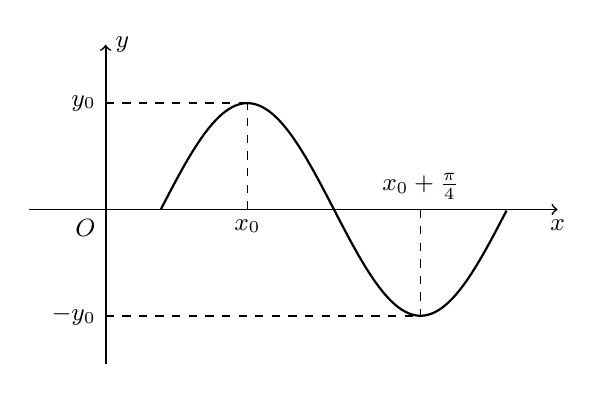
\begin{tikzpicture}[semithick, font=\small, x=2.8cm, y=1.35cm]
  \def\xz{0.6427}   % x0，最高点
  \def\xm{1.4284}   % x0+π/4，最低点
  \def\xs{0.25}     % 图象左端与 x 轴的交点
  % 坐标轴
  \draw[->] (-0.35,0) -- (2.05,0) node[below] {$x$};
  \draw[->] (0,-1.45) -- (0,1.55) node[right] {$y$};
  \node[below left] at (0,0) {$O$};
  % 最高点、最低点的虚线
  \draw[dashed] (0,1) -- (\xz,1);
  \draw[dashed] (\xz,0) -- (\xz,1);
  \draw[dashed] (0,-1) -- (\xm,-1);
  \draw[dashed] (\xm,0) -- (\xm,-1);
  % 正弦曲线
  \draw[thick, domain=\xs:1.8208, samples=240, smooth]
    plot (\x, {sin(4*(\x-\xs) r)});
  % 标注
  \node[left] at (0,1) {$y_0$};
  \node[left] at (0,-1) {$-y_0$};
  \node[below] at (\xz,0) {$x_0$};
  \node[above] at (\xm,0) {$x_0+\frac{\pi}{4}$};
\end{tikzpicture}
\end{center}
\nopagebreak[4]
（A）$5$；（B）$4$；（C）$3$；（D）$2$。

\Needspace{4\baselineskip}
\textbf{解析}
\Needspace{5\baselineskip}
由图读出：图象的最高点为 $(x_0,y_0)$，最低点为 $\left(x_0+\dfrac\pi4,-y_0\right)$。相邻的最高点与最低点横坐标之差等于半个周期，故
\nopagebreak[4]
\[\frac T2=\left(x_0+\frac\pi4\right)-x_0=\frac\pi4,\]
\Needspace{5\baselineskip}
从而 $T=\dfrac\pi2$。又 $\omega>0$，所以
\nopagebreak[4]
\[\omega=\frac{2\pi}T=\frac{2\pi}{\pi/2}=4.\]
选 B。

\gkanswer{答案：B。}

\end{answer}
\begin{answer}
\gksolhead{10}{}

\textbf{题目}：

已知曲线 $y=x^4+ax^2+1$ 在点 $(-1,a+2)$ 处切线的斜率为 $8$，则 $a=$\mbox{（　　）}

（A）$9$；（B）$6$；（C）$-9$；（D）$-6$。

\Needspace{4\baselineskip}
\textbf{解析}
\Needspace{5\baselineskip}
对 $y=x^4+ax^2+1$ 求导：
\nopagebreak[4]
\[y'=4x^3+2ax.\]
\Needspace{5\baselineskip}
在 $x=-1$ 处切线斜率为 $8$，故
\nopagebreak[4]
\[4(-1)^3+2a(-1)=8\Longrightarrow -4-2a=8,\]
解得 $a=-6$。选 D。

\gkanswer{答案：D。}

\end{answer}
\begin{answer}
\gksolhead{11}{}

\textbf{题目}：

已知正四棱柱 $ABCD\text{-}A_1B_1C_1D_1$ 中，$AA_1=2AB$，则 $CD$ 与平面 $BDC_1$ 所成角的正弦值等于\mbox{（　　）}

（A）$\dfrac23$；（B）$\dfrac{\sqrt3}3$；（C）$\dfrac{\sqrt2}3$；（D）$\dfrac13$。

\Needspace{4\baselineskip}
\textbf{解析}
\Needspace{5\baselineskip}
设 $AB=1$，则 $AA_1=2$。以 $A$ 为原点，$AB$，$AD$，$AA_1$ 所在直线分别为 $x$，$y$，$z$ 轴建立坐标系：
\nopagebreak[4]
\[A(0,0,0),\quad B(1,0,0),\quad D(0,1,0),\]
\nopagebreak[4]
\[C(1,1,0),\quad C_1(1,1,2).\]
\Needspace{5\baselineskip}
平面 $BDC_1$ 内两向量
\nopagebreak[4]
\[\overrightarrow{DB}=(1,-1,0),\qquad
\overrightarrow{DC_1}=(1,0,2).\]
\Needspace{5\baselineskip}
其法向量可取
\nopagebreak[4]
\[\boldsymbol n=\overrightarrow{DB}\times\overrightarrow{DC_1}
=(-2,-2,1),\qquad|\boldsymbol n|=3.\]
\Needspace{5\baselineskip}
又 $CD$ 的方向向量
\nopagebreak[4]
\[\overrightarrow{CD}=(-1,0,0).\]
\Needspace{5\baselineskip}
设 $CD$ 与平面 $BDC_1$ 所成角为 $\theta$，则
\nopagebreak[4]
\[\sin\theta
=\frac{\left|\overrightarrow{CD}\cdot\boldsymbol n\right|}
{|\overrightarrow{CD}|\,|\boldsymbol n|}
=\frac{2}{1\times3}=\frac23.\]
选 A。

\gkanswer{答案：A。}

\end{answer}
\begin{answer}
\gksolhead{12}{}

\textbf{题目}：

已知抛物线 $C:y^2=8x$ 与点 $M(-2,2)$，过 $C$ 的焦点且斜率为 $k$ 的直线与 $C$ 交于 $A$、$B$ 两点，若 $\overrightarrow{MA}\cdot\overrightarrow{MB}=0$，则 $k=$\mbox{（　　）}

（A）$\dfrac12$；（B）$\dfrac{\sqrt2}2$；（C）$\sqrt2$；（D）$2$。

\Needspace{4\baselineskip}
\textbf{解析}
\Needspace{5\baselineskip}
抛物线 $y^2=8x$ 的焦点为 $F(2,0)$。过 $F$ 且斜率为 $k$ 的直线为
\nopagebreak[4]
\[y=k(x-2)\quad(k\neq0).\]
\Needspace{5\baselineskip}
代入 $y^2=8x$：
\nopagebreak[4]
\[k^2(x-2)^2=8x,\]
\Needspace{5\baselineskip}
即
\nopagebreak[4]
\[k^2x^2-(4k^2+8)x+4k^2=0.\]
\Needspace{5\baselineskip}
设 $A(x_1,y_1)$，$B(x_2,y_2)$，由韦达定理
\nopagebreak[4]
\[x_1+x_2=\frac{4k^2+8}{k^2}=4+\frac8{k^2},\qquad
x_1x_2=4.\]
\Needspace{5\baselineskip}
由 $\overrightarrow{MA}\cdot\overrightarrow{MB}=0$ 得
\nopagebreak[4]
\[(x_1+2)(x_2+2)+(y_1-2)(y_2-2)=0.\]
\Needspace{5\baselineskip}
先算第一部分：
\nopagebreak[4]
\[(x_1+2)(x_2+2)=x_1x_2+2(x_1+x_2)+4
=16+\frac{16}{k^2}.\]
\Needspace{5\baselineskip}
又 $y_i-2=k(x_i-2)-2$，故
\nopagebreak[4]
\[\begin{aligned}
(y_1-2)(y_2-2)
&=k^2(x_1-2)(x_2-2)\\
&\quad-2k\left[(x_1-2)+(x_2-2)\right]+4.
\end{aligned}\]
\Needspace{5\baselineskip}
其中
\nopagebreak[4]
\[(x_1-2)(x_2-2)=4-2\left(4+\frac8{k^2}\right)+4
=-\frac{16}{k^2},\]
\nopagebreak[4]
\[(x_1-2)+(x_2-2)=4+\frac8{k^2}-4=\frac8{k^2}.\]
\Needspace{5\baselineskip}
所以
\nopagebreak[4]
\[(y_1-2)(y_2-2)
=-16-\frac{16}{k}+4=-12-\frac{16}{k}.\]
\Needspace{5\baselineskip}
代入点积条件：
\nopagebreak[4]
\[16+\frac{16}{k^2}-12-\frac{16}{k}=0,\]
\Needspace{5\baselineskip}
两边乘以 $k^2$ 得
\nopagebreak[4]
\[4k^2-16k+16=0\Longrightarrow (k-2)^2=0,\]
故 $k=2$。选 D。

\gkanswer{答案：D。}

\end{answer}
\begin{answer}
\gksolhead{13}{}

\textbf{题目}：

设 $f(x)$ 是以 $2$ 为周期的函数，且当 $x\in[1,3)$ 时，$f(x)=x-2$，则 $f(-1)=$\gkblank{}。

\Needspace{4\baselineskip}
\textbf{解析}
\Needspace{5\baselineskip}
$f(x)$ 以 $2$ 为周期，故
\nopagebreak[4]
\[f(-1)=f(-1+2)=f(1).\]
\Needspace{5\baselineskip}
因为 $1\in[1,3)$，由该区间上的表达式得
\nopagebreak[4]
\[f(1)=1-2=-1.\]
所以 $f(-1)=-1$。

\gkanswer{答案：$-1$。}

\end{answer}
\begin{answer}
\gksolhead{14}{}

\textbf{题目}：

从进入决赛的 $6$ 名选手中决出 $1$ 名一等奖，$2$ 名二等奖，$3$ 名三等奖，则可能的决赛结果共有\gkblank{}种。（用数字作答）

\Needspace{4\baselineskip}
\textbf{解析}
\Needspace{5\baselineskip}
先从 $6$ 人中选 $1$ 人为一等奖，再从剩下 $5$ 人中选 $2$ 人为二等奖，其余 $3$ 人自动为三等奖：
\nopagebreak[4]
\[\mathrm C_6^1\mathrm C_5^2\mathrm C_3^3
=6\times10\times1=60.\]
故可能的决赛结果共有 $60$ 种。

\gkanswer{答案：$60$。}

\end{answer}
\begin{answer}
\gksolhead{15}{}

\textbf{题目}：

若 $x$，$y$ 满足约束条件 $\begin{cases}x\geqslant0,\\ x+3y\geqslant4,\\ 3x+y\leqslant4,\end{cases}$ 则 $z=-x+y$ 的最小值为\gkblank{}。

\Needspace{4\baselineskip}
\textbf{解析}
\Needspace{5\baselineskip}
画出可行域。三条边界直线
\nopagebreak[4]
\[x=0,\qquad x+3y=4,\qquad 3x+y=4\]
\Needspace{5\baselineskip}
的两两交点为
\nopagebreak[4]
\[\left(0,\frac43\right),\qquad(1,1),\qquad(0,4).\]
\Needspace{5\baselineskip}
其中 $(1,1)$ 是后两条直线的交点，$(0,4)$ 是 $x=0$ 与 $3x+y=4$ 的交点。可行域是以这三点为顶点的三角形。分别计算
\nopagebreak[4]
\[z=-x+y\]
\Needspace{5\baselineskip}
在三个顶点处的值：
\nopagebreak[4]
\[z\left(0,\frac43\right)=\frac43,\qquad
z(1,1)=0,\qquad z(0,4)=4.\]
线性函数在可行域上的最值在顶点处取得，故最小值为 $0$。

\gkanswer{答案：$0$。}

\end{answer}
\begin{answer}
\gksolhead{16}{}

\textbf{题目}：

已知圆 $O$ 和圆 $K$ 是球 $O$ 的大圆和小圆，其公共弦长等于球 $O$ 的半径，$OK=\dfrac32$，且圆 $O$ 与圆 $K$ 所在的平面所成的一个二面角为 $60^\circ$，则球 $O$ 的表面积等于\gkblank{}。

\Needspace{4\baselineskip}
\textbf{解析}
\Needspace{5\baselineskip}
设球 $O$ 的半径为 $R$，圆 $O$ 为大圆，圆 $K$ 为小圆，两圆所在平面的公共弦为 $AB$，其中点为 $M$。则 $AB=R$，且
\nopagebreak[4]
\[OM\perp AB,\qquad KM\perp AB.\]
又 $OK$ 垂直于小圆 $K$ 所在平面，而 $AB$ 在该平面内，故 $OK\perp AB$。于是 $OK\perp KM$，三角形 $OKM$ 在 $K$ 处为直角。

\Needspace{5\baselineskip}
对 $AB$ 上任意点 $X$，因 $OK\perp KX$，有
\nopagebreak[4]
\[OX^2=OK^2+KX^2.\]
\Needspace{5\baselineskip}
故 $OX$ 最小时 $KX$ 也最小，$O$ 到 $AB$ 的垂足与 $K$ 到 $AB$ 的垂足同为 $M$，从而
\nopagebreak[4]
\[OM^2=OK^2+KM^2.\]
\Needspace{5\baselineskip}
两平面所成的二面角等于 $OM$ 与 $KM$ 的夹角。由 $OK\perp KM$ 知 $\angle OMK$ 为锐角，故
\nopagebreak[4]
\[\angle OMK=60^\circ.\]
\Needspace{5\baselineskip}
在直角三角形 $OMK$ 中，
\nopagebreak[4]
\[OM=\frac{OK}{\sin60^\circ}
=\frac{3/2}{\sqrt3/2}=\sqrt3.\]
\Needspace{5\baselineskip}
大圆中弦 $AB=R$，弦心距 $OM=\dfrac{\sqrt3R}{2}$，所以
\nopagebreak[4]
\[\frac{\sqrt3R}{2}=\sqrt3\Longrightarrow R=2.\]
\Needspace{5\baselineskip}
球 $O$ 的表面积
\nopagebreak[4]
\[S=4\pi R^2=4\pi\times4=16\pi.\]

\gkanswer{答案：$16\pi$。}

\end{answer}
\begin{answer}
\gksolhead{17}{}

\textbf{题目}：

等差数列 $\{a_n\}$ 中，$a_7=4$，$a_{19}=2a_9$。

（1） 求 $\{a_n\}$ 的通项公式；

（2） 设 $b_n=\dfrac1{na_n}$，求数列 $\{b_n\}$ 的前 $n$ 项和 $S_n$。

\Needspace{4\baselineskip}
\textbf{解析}
\Needspace{5\baselineskip}
\textbf{（1）} 设等差数列 $\{a_n\}$ 的公差为 $d$。由 $a_7=4$ 得
\nopagebreak[4]
\[a_1+6d=4.\]
\Needspace{5\baselineskip}
由 $a_{19}=2a_9$ 得
\nopagebreak[4]
\[a_1+18d=2(a_1+8d),\]
\Needspace{5\baselineskip}
即
\nopagebreak[4]
\[a_1+18d=2a_1+16d\Longrightarrow a_1=2d.\]
\Needspace{5\baselineskip}
代入 $a_1+6d=4$：
\nopagebreak[4]
\[8d=4\Longrightarrow d=\frac12,\qquad a_1=1.\]
\Needspace{5\baselineskip}
故
\nopagebreak[4]
\[a_n=1+(n-1)\cdot\frac12=\frac{n+1}2\quad(n\in\mathbf N^*).\]

\Needspace{5\baselineskip}
\textbf{（2）} 由（1）得
\nopagebreak[4]
\[b_n=\frac1{na_n}
=\frac1{n\cdot\frac{n+1}2}
=\frac2{n(n+1)}
=2\left(\frac1n-\frac1{n+1}\right).\]
\Needspace{5\baselineskip}
所以
\nopagebreak[4]
\[\begin{aligned}
S_n&=\sum_{k=1}^{n}b_k
=2\sum_{k=1}^{n}\left(\frac1k-\frac1{k+1}\right)\\
&=2\left(1-\frac1{n+1}\right)
=\frac{2n}{n+1}.
\end{aligned}\]

\gkanswer{答案（1）：$a_n=\dfrac{n+1}2$（$n\in\mathbf N^*$）。}

\gkanswer{答案（2）：$S_n=\dfrac{2n}{n+1}$。}

\end{answer}
\begin{answer}
\gksolhead{18}{}

\textbf{题目}：

设 $\triangle ABC$ 的内角 $A$，$B$，$C$ 的对边分别为 $a$，$b$，$c$，$(a+b+c)(a-b+c)=ac$。

（1） 求 $B$；

（2） 若 $\sin A\sin C=\dfrac{\sqrt3-1}4$，求 $C$。

\Needspace{4\baselineskip}
\textbf{解析}
\Needspace{5\baselineskip}
\textbf{（1）} 展开条件左边：
\nopagebreak[4]
\[\begin{aligned}
(a+b+c)(a-b+c)
&=(a+c)^2-b^2\\
&=a^2+2ac+c^2-b^2.
\end{aligned}\]
\Needspace{5\baselineskip}
由条件它等于 $ac$，故
\nopagebreak[4]
\[a^2+c^2-b^2=-ac.\]
\Needspace{5\baselineskip}
于是由余弦定理
\nopagebreak[4]
\[\cos B=\frac{a^2+c^2-b^2}{2ac}
=\frac{-ac}{2ac}=-\frac12.\]
\Needspace{5\baselineskip}
因 $0<B<\pi$，故
\nopagebreak[4]
\[B=\frac{2\pi}3.\]

\Needspace{5\baselineskip}
\textbf{（2）} 由（1），
\nopagebreak[4]
\[A+C=\pi-B=\frac\pi3.\]
\Needspace{5\baselineskip}
利用积化和差，
\nopagebreak[4]
\[\sin A\sin C
=\frac{\cos(A-C)-\cos(A+C)}2
=\frac{\cos(A-C)-\frac12}{2}.\]
\Needspace{5\baselineskip}
由条件
\nopagebreak[4]
\[\frac{\cos(A-C)-\frac12}{2}=\frac{\sqrt3-1}{4},\]
\Needspace{5\baselineskip}
故
\nopagebreak[4]
\[\cos(A-C)-\frac12=\frac{\sqrt3-1}{2}
\Longrightarrow \cos(A-C)=\frac{\sqrt3}{2}.\]
\Needspace{5\baselineskip}
因为 $A>0$，$C>0$ 且 $A+C=\dfrac\pi3$，所以
\nopagebreak[4]
\[-\frac\pi3<A-C<\frac\pi3.\]
\Needspace{5\baselineskip}
在此范围内 $\cos(A-C)=\dfrac{\sqrt3}{2}$ 给出
\nopagebreak[4]
\[A-C=\pm\frac\pi6.\]
\Needspace{5\baselineskip}
若 $A-C=\dfrac\pi6$，联立 $A+C=\dfrac\pi3$ 得
\nopagebreak[4]
\[A=\frac\pi4,\qquad C=\frac{\pi}{12}.\]
\Needspace{5\baselineskip}
若 $A-C=-\dfrac\pi6$，则
\nopagebreak[4]
\[C=\frac\pi4.\]
\Needspace{5\baselineskip}
故
\nopagebreak[4]
\[C=\frac{\pi}{12}\quad\text{\text{或}}\quad C=\frac\pi4.\]

\gkanswer{答案（1）：$B=\dfrac{2\pi}3$。}

\gkanswer{答案（2）：$C=\dfrac{\pi}{12}$ 或 $C=\dfrac\pi4$。}

\end{answer}
\begin{answer}
\gksolhead{19}{}

\textbf{题目}：

如图，四棱锥 $P\text{-}ABCD$ 中，$\angle ABC=\angle BAD=90^\circ$，$BC=2AD$，$\triangle PAB$ 与 $\triangle PAD$ 都是边长为 $2$ 的等边三角形。

（1） 证明：$PB\perp CD$；

（2） 求点 $A$ 到平面 $PCD$ 的距离。
\nopagebreak[4]
\begin{center}% 2013 年全国大纲卷文科第 19 题：四棱锥 P-ABCD。
% 来源 PDF：普通高考/2013/2013大纲文(广西).pdf，第 1 页（印面 797）右栏。
% 底面为直角梯形，AD∥BC，∠ABC=∠BAD=90°；CD、DA、PD 被遮挡。
\begin{tikzpicture}[semithick, font=\small]
  \coordinate (C) at (0.6,0.9);
  \coordinate (B) at (8.2,0.9);
  \coordinate (A) at (9.4,2.6);
  \coordinate (D) at (5.4,2.6);
  \coordinate (P) at (6.0,6.2);
  % 可见棱
  \draw (P) -- (C);
  \draw (P) -- (B);
  \draw (P) -- (A);
  \draw (C) -- (B) -- (A);
  % 被遮挡的棱
  \draw[dashed] (P) -- (D);
  \draw[dashed] (C) -- (D) -- (A);
  % 标注
  \node[above] at (P) {$P$};
  \node[right] at (A) {$A$};
  \node[below] at (B) {$B$};
  \node[below left] at (C) {$C$};
  \node[above left] at (D) {$D$};
\end{tikzpicture}
\end{center}
\nopagebreak[4]
\Needspace{4\baselineskip}
\textbf{解析}
\textbf{（1）} 因为 $\angle ABC=\angle BAD=90^\circ$，所以 $AB\perp BC$，$AB\perp AD$。又 $AD$，$BC$ 都在底面内，故 $AD\parallel BC$。由 $BC=2AD$ 且等边三角形边长给出 $AD=AB=2$，所以 $BC=4$。

\Needspace{5\baselineskip}
以 $A$ 为原点，$AB$，$AD$ 所在直线分别为 $x$，$y$ 轴，过 $A$ 垂直于底面的直线为 $z$ 轴建立坐标系：
\nopagebreak[4]
\[A(0,0,0),\quad B(2,0,0),\quad D(0,2,0).\]
\Needspace{5\baselineskip}
由 $AD\parallel BC$ 且 $BC=4$，结合图形中 $C$，$D$ 在 $AB$ 同侧，得
\nopagebreak[4]
\[C(2,4,0).\]
\Needspace{5\baselineskip}
设 $P(x,y,z)$。由 $PA=PB=PD=2$：
\nopagebreak[4]
\[x^2+y^2+z^2=4,\]
\nopagebreak[4]
\[(x-2)^2+y^2+z^2=4\Longrightarrow x=1,\]
\nopagebreak[4]
\[x^2+(y-2)^2+z^2=4\Longrightarrow y=1.\]
\Needspace{5\baselineskip}
于是 $z^2=4-1-1=2$，取 $z=\sqrt2$，得
\nopagebreak[4]
\[P(1,1,\sqrt2).\]
（取 $z=-\sqrt2$ 只把图形关于底面对称，不影响以下结论。）

\Needspace{5\baselineskip}
计算
\nopagebreak[4]
\[\overrightarrow{PB}=(1,-1,-\sqrt2),\qquad
\overrightarrow{CD}=(-2,-2,0).\]
\Needspace{5\baselineskip}
则
\nopagebreak[4]
\[\overrightarrow{PB}\cdot\overrightarrow{CD}
=1\times(-2)+(-1)\times(-2)+0=0.\]
故 $PB\perp CD$。

\Needspace{5\baselineskip}
\textbf{（2）} 平面 $PCD$ 内两向量
\nopagebreak[4]
\[\overrightarrow{DC}=(2,2,0),\qquad
\overrightarrow{DP}=(1,-1,\sqrt2).\]
\Needspace{5\baselineskip}
其法向量可取
\nopagebreak[4]
\[\boldsymbol n=\overrightarrow{DC}\times\overrightarrow{DP}
=(2\sqrt2,-2\sqrt2,-4).\]
\Needspace{5\baselineskip}
化简可取 $\boldsymbol n=(\sqrt2,-\sqrt2,-2)$。平面过 $D(0,2,0)$，故方程为
\nopagebreak[4]
\[\sqrt2x-\sqrt2(y-2)-2z=0,\]
\Needspace{5\baselineskip}
即
\nopagebreak[4]
\[\sqrt2x-\sqrt2y+2\sqrt2-2z=0.\]
\Needspace{5\baselineskip}
点 $A(0,0,0)$ 到该平面的距离为
\nopagebreak[4]
\[d=\frac{|2\sqrt2|}
{\sqrt{(\sqrt2)^2+(-\sqrt2)^2+(-2)^2}}
=\frac{2\sqrt2}{\sqrt8}=1.\]
故点 $A$ 到平面 $PCD$ 的距离为 $1$。

\gkanswer{答案（1）：证明见解析。}

\gkanswer{答案（2）：$1$。}

\end{answer}
\begin{answer}
\gksolhead{20}{}

\textbf{题目}：

甲、乙、丙三人进行羽毛球练习赛，其中两人比赛，另一人当裁判，每局比赛结束时，负的一方在下一局当裁判。设各局中双方获胜的概率均为 $\dfrac12$，各局比赛的结果都相互独立，第 $1$ 局甲当裁判。

（1） 求第 $4$ 局甲当裁判的概率；

（2） 求前 $4$ 局中乙恰好当 $1$ 次裁判的概率。

\Needspace{4\baselineskip}
\textbf{解析}
\Needspace{5\baselineskip}
设第 $n$ 局的裁判为 $J_n$。已知 $J_1=$ 甲。每局由另外两人比赛，负者担任下一局裁判，故 $J_{n+1}$ 是第 $n$ 局两名比赛者之一。由于第 $n$ 局的两名比赛者恰为除 $J_n$ 外的另外两人，且两人获胜概率各为 $\dfrac12$，所以
\nopagebreak[4]
\[P(J_{n+1}=X\mid J_n)=
\begin{cases}
\dfrac12,&X\neq J_n,\\
0,&X=J_n.
\end{cases}\]
也就是说，下一局裁判在另外两人中等可能选取。

\Needspace{5\baselineskip}
\textbf{（1）} 先求第 3 局裁判的分布。由 $J_1=$ 甲，
\nopagebreak[4]
\[P(J_2=\text{\text{乙}})=P(J_2=\text{\text{丙}})=\frac12.\]
\Needspace{5\baselineskip}
若 $J_2=$ 乙，则 $J_3$ 等可能为甲或丙；若 $J_2=$ 丙，则 $J_3$ 等可能为甲或乙。故
\nopagebreak[4]
\[P(J_3=\text{\text{甲}})=\frac12,\]
\nopagebreak[4]
\[P(J_3=\text{\text{乙}})=P(J_3=\text{\text{丙}})=\frac14.\]
\Needspace{5\baselineskip}
第 4 局甲当裁判，必须 $J_3$ 为乙或丙，且由 $J_3$ 转移到甲的概率为 $\dfrac12$：
\nopagebreak[4]
\[\begin{aligned}
P(J_4=\text{\text{甲}})
&=P(J_3=\text{\text{乙}})\cdot\frac12
+P(J_3=\text{\text{丙}})\cdot\frac12\\
&=\frac14\cdot\frac12+\frac14\cdot\frac12=\frac14.
\end{aligned}\]

\textbf{（2）} 第 1 局甲当裁判，故只需在前 $3$ 局（第 $2$，$3$，$4$ 局）中乙恰好当 $1$ 次裁判。仍按 $J_2$ 分类。

\Needspace{5\baselineskip}
若 $J_2=$ 乙，概率为 $\dfrac12$。此时 $J_3$ 为甲或丙，无论哪种，$J_4$ 不等于乙的概率都是 $\dfrac12$，故这一支贡献
\nopagebreak[4]
\[\frac12\cdot\frac12=\frac14.\]

若 $J_2=$ 丙，概率为 $\dfrac12$。此时 $J_3$ 等可能为甲或乙。若 $J_3=$ 乙，其概率为 $\dfrac12$，而 $J_4$ 只能为甲或丙，必不等于乙，这一支贡献 $\dfrac12\cdot\dfrac12=\dfrac14$。若 $J_3=$ 甲，其概率为 $\dfrac12$，此时要恰有 $1$ 次乙，必须 $J_4=$ 乙，概率为 $\dfrac12$，这一支贡献 $\dfrac12\cdot\dfrac12\cdot\dfrac12=\dfrac18$。

\Needspace{5\baselineskip}
三部分互斥，故所求概率为
\nopagebreak[4]
\[\frac14+\frac14+\frac18=\frac58.\]

\gkanswer{答案（1）：$\dfrac14$。}

\gkanswer{答案（2）：$\dfrac58$。}

\end{answer}
\begin{answer}
\gksolhead{21}{}

\textbf{题目}：

已知函数 $f(x)=x^3+3ax^2+3x+1$。

（1） 当 $a=-\sqrt2$ 时，讨论 $f(x)$ 的单调性；

（2） 若 $x\in[2,+\infty)$ 时，$f(x)\geqslant0$，求 $a$ 的取值范围。

\Needspace{4\baselineskip}
\textbf{解析}
\Needspace{5\baselineskip}
\textbf{（1）} 求导：
\nopagebreak[4]
\[f'(x)=3x^2+6ax+3=3(x^2+2ax+1).\]
\Needspace{5\baselineskip}
当 $a=-\sqrt2$ 时，
\nopagebreak[4]
\[x^2+2ax+1=x^2-2\sqrt2x+1
=\left(x-(\sqrt2-1)\right)\left(x-(\sqrt2+1)\right).\]
\Needspace{5\baselineskip}
即
\nopagebreak[4]
\[f'(x)=3\left(x-(\sqrt2-1)\right)\left(x-(\sqrt2+1)\right).\]
\Needspace{5\baselineskip}
因为 $\sqrt2-1<\sqrt2+1$，所以
\nopagebreak[4]
\[f'(x)>0\quad\text{\text{当} }x<\sqrt2-1\text{ \text{或} }x>\sqrt2+1,\]
\nopagebreak[4]
\[f'(x)<0\quad\text{\text{当} }\sqrt2-1<x<\sqrt2+1.\]
故 $f(x)$ 在 $\left(-\infty,\sqrt2-1\right)$ 与 $\left(\sqrt2+1,+\infty\right)$ 上单调递增，在 $\left(\sqrt2-1,\sqrt2+1\right)$ 上单调递减。

\Needspace{5\baselineskip}
\textbf{（2）} 当 $x\geqslant2$ 时，$x^2>0$，将 $f(x)$ 变形：
\nopagebreak[4]
\[f(x)=3x^2\left[a+\frac{x^3+3x+1}{3x^2}\right].\]
\Needspace{5\baselineskip}
记
\nopagebreak[4]
\[h(x)=\frac{x^3+3x+1}{3x^2}
=\frac x3+\frac1x+\frac1{3x^2}.\]
\Needspace{5\baselineskip}
则 $f(x)\geqslant0$ 等价于
\nopagebreak[4]
\[a\geqslant-h(x)\quad\text{\text{对一切} }x\geqslant2\text{ \text{成立}}.\]
\Needspace{5\baselineskip}
求导：
\nopagebreak[4]
\[\begin{aligned}
h'(x)&=\frac13-\frac1{x^2}-\frac2{3x^3}\\
&=\frac{x^3-3x-2}{3x^3}
=\frac{(x-2)(x+1)^2}{3x^3}.
\end{aligned}\]
\Needspace{5\baselineskip}
当 $x\geqslant2$ 时，$h'(x)\geqslant0$，故 $h(x)$ 在 $[2,+\infty)$ 上单调递增，从而 $-h(x)$ 单调递减，其最大值为
\nopagebreak[4]
\[-h(2)=-\left(\frac23+\frac12+\frac1{12}\right)
=-\frac{15}{12}=-\frac54.\]
\Needspace{5\baselineskip}
因此要使 $a\geqslant-h(x)$ 对一切 $x\geqslant2$ 成立，必须且只需
\nopagebreak[4]
\[a\geqslant-\frac54.\]
\Needspace{5\baselineskip}
即 $a$ 的取值范围为
\nopagebreak[4]
\[\left[-\frac54,+\infty\right).\]

\gkanswer{答案（1）：$f(x)$ 在 $\left(-\infty,\sqrt2-1\right)$ 与 $\left(\sqrt2+1,+\infty\right)$ 上单调递增，在 $\left(\sqrt2-1,\sqrt2+1\right)$ 上单调递减。}

\gkanswer{答案（2）：$\left[-\dfrac54,+\infty\right)$。}

\end{answer}
\begin{answer}
\gksolhead{22}{}

\textbf{题目}：

已知双曲线 $C:\dfrac{x^2}{a^2}-\dfrac{y^2}{b^2}=1$（$a>0$，$b>0$）的左、右焦点分别为 $F_1$、$F_2$，离心率为 $3$，直线 $y=2$ 与 $C$ 的两个交点间的距离为 $\sqrt6$。

（1） 求 $a$、$b$；

（2） 设过 $F_2$ 的直线 $l$ 与 $C$ 的左、右两支分别交于 $A$、$B$ 两点，且 $|AF_1|=|BF_1|$，证明：$|AF_2|$、$|AB|$、$|BF_2|$ 成等比数列。

\Needspace{4\baselineskip}
\textbf{解析}
\Needspace{5\baselineskip}
\textbf{（1）} 由离心率
\nopagebreak[4]
\[e=\frac ca=3\Longrightarrow c=3a,\]
\Needspace{5\baselineskip}
故
\nopagebreak[4]
\[b^2=c^2-a^2=9a^2-a^2=8a^2.\]
\Needspace{5\baselineskip}
在 $y=2$ 处，代入双曲线方程：
\nopagebreak[4]
\[\frac{x^2}{a^2}-\frac4{b^2}=1
\Longrightarrow \frac{x^2}{a^2}=1+\frac4{8a^2}
=1+\frac1{2a^2}.\]
\Needspace{5\baselineskip}
所以
\nopagebreak[4]
\[x^2=a^2+\frac12.\]
\Needspace{5\baselineskip}
两个交点为 $\left(\pm\sqrt{a^2+\frac12},2\right)$，其距离为
\nopagebreak[4]
\[2\sqrt{a^2+\frac12}=\sqrt6.\]
\Needspace{5\baselineskip}
平方得
\nopagebreak[4]
\[4\left(a^2+\frac12\right)=6
\Longrightarrow a^2+\frac12=\frac32
\Longrightarrow a^2=1.\]
\Needspace{5\baselineskip}
故 $a=1$，$b^2=8$，即
\nopagebreak[4]
\[a=1,\qquad b=2\sqrt2.\]

\Needspace{5\baselineskip}
\textbf{（2）} 由（1），$c=3$，焦点为
\nopagebreak[4]
\[F_1(-3,0),\qquad F_2(3,0).\]
\Needspace{5\baselineskip}
直线 $l$ 过 $F_2$ 且与左、右两支各交于一点，故 $l$ 不可能是竖直线 $x=3$（它与右支交于两点）。设
\nopagebreak[4]
\[l:\ y=k(x-3).\]
\Needspace{5\baselineskip}
代入 $x^2-\dfrac{y^2}8=1$：
\nopagebreak[4]
\[8x^2-k^2(x-3)^2=8,\]
\Needspace{5\baselineskip}
整理得
\nopagebreak[4]
\[(8-k^2)x^2+6k^2x-9k^2-8=0.\]
\Needspace{5\baselineskip}
设 $A(x_A,y_A)$ 在左支，$B(x_B,y_B)$ 在右支，则 $x_A<0<x_B$，且由韦达定理
\nopagebreak[4]
\[x_A+x_B=-\frac{6k^2}{8-k^2},\qquad
x_Ax_B=\frac{-9k^2-8}{8-k^2}.\]

\Needspace{5\baselineskip}
对左支上的 $A$，焦半径公式为
\nopagebreak[4]
\[|AF_1|=-3x_A-1,\qquad |AF_2|=-3x_A+1.\]
\Needspace{5\baselineskip}
对右支上的 $B$，焦半径公式为
\nopagebreak[4]
\[|BF_1|=3x_B+1,\qquad |BF_2|=3x_B-1.\]
\Needspace{5\baselineskip}
由 $|AF_1|=|BF_1|$ 得
\nopagebreak[4]
\[-3x_A-1=3x_B+1
\Longrightarrow x_A+x_B=-\frac23.\]
\Needspace{5\baselineskip}
与韦达定理比较：
\nopagebreak[4]
\[-\frac{6k^2}{8-k^2}=-\frac23
\Longrightarrow 18k^2=16-2k^2,\]
\Needspace{5\baselineskip}
故
\nopagebreak[4]
\[k^2=\frac45.\]
\Needspace{5\baselineskip}
此时
\nopagebreak[4]
\[x_Ax_B
=\frac{-9\cdot\frac45-8}{8-\frac45}
=\frac{-\frac{36}5-8}{\frac{36}5}
=-\frac{19}9.\]
\Needspace{5\baselineskip}
于是 $x_B$ 是方程
\nopagebreak[4]
\[x^2+\frac23x-\frac{19}9=0\]
\Needspace{5\baselineskip}
的根，即
\nopagebreak[4]
\[9x_B^2+6x_B-19=0.\]
\Needspace{5\baselineskip}
令 $t=|AF_1|=|BF_1|=3x_B+1$。由焦半径公式
\nopagebreak[4]
\[|AF_2|=t+2,\qquad |BF_2|=t-2,\]
\Needspace{5\baselineskip}
故
\nopagebreak[4]
\[\begin{aligned}
|AF_2|\cdot|BF_2|
&=(t+2)(t-2)=t^2-4\\
&=(3x_B+1)^2-4\\
&=9x_B^2+6x_B-3\\
&=19-3=16.
\end{aligned}\]
\Needspace{5\baselineskip}
另一方面，
\nopagebreak[4]
\[\begin{aligned}
|AB|^2
&=(1+k^2)(x_A-x_B)^2\\
&=\left(1+\frac45\right)
\left[(x_A+x_B)^2-4x_Ax_B\right]\\
&=\frac95\left(\frac49+\frac{76}9\right)
=\frac95\cdot\frac{80}9=16.
\end{aligned}\]
\Needspace{5\baselineskip}
所以
\nopagebreak[4]
\[|AB|^2=|AF_2|\cdot|BF_2|,\]
\Needspace{5\baselineskip}
即
\nopagebreak[4]
\[\frac{|AB|}{|AF_2|}=\frac{|BF_2|}{|AB|}.\]
又 $|AF_2|$，$|AB|$，$|BF_2|$ 均为正数，故 $|AF_2|$，$|AB|$，$|BF_2|$ 成等比数列。

\gkanswer{答案（1）：$a=1$，$b=2\sqrt2$。}

\gkanswer{答案（2）：证明见解析。}

\end{answer}